         \chapter{States of matter and the kinetic molecular theory}\fancyfoot[LO,RE]{Chemistry: Matter and Materials}
    \setcounter{figure}{1}
    \setcounter{subfigure}{1}
% \label{m38736*cid1}
%             \section{ Introduction}
%             \nopagebreak
\label{m38736*cid2}
            \section{States of matter}
            \nopagebreak
            \label{m38736} $ \hspace{-5pt}\begin{array}{cccccccccccc}   \end{array} $ \hspace{2 pt}\raisebox{-5 pt}{
\includegraphics[width=0.5cm]{col11305.imgs/summary_www.png}} {(section shortcode: P10014 )} \par 

\label{m38736*id802341}In this chapter we will explore the states of matter and then look at the kinetic molecular theory. Matter exists in three states: solid, liquid and gas. We will also examine how the kinetic theory of matter helps explain boiling and melting points as well as other properties of matter.\par 

\label{m38736*id324876121}All matter is made up of particles. We can see this when we look at diffusion. \par
\Definition{Diffusion}{Diffusion is the movement of particles from a high concentration to a low concentration.} 
\begin{minipage}{.5\textwidth}
Diffusion can be seen as a spreading out of particles resulting in an even distribution of the particles. You can see diffusion when you place a drop of food colouring in water. The colour slowly spreads out through the water. If matter were not made of particles that are constantly moving then we would only see a clump of colour when we put the food colouring in water, as there would be nothing that could move about and mix in with the water.
\end{minipage}
\begin{minipage}{.5\textwidth}
\begin{center}
 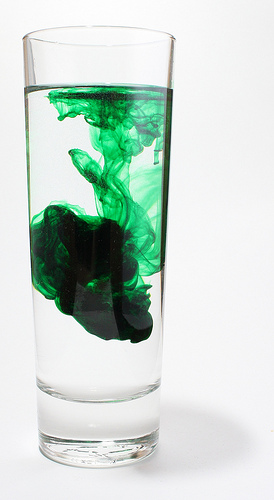
\includegraphics[height=.5\textwidth]{photos/diffusionby-LadyDayDream-flickr.jpg}\par
\textit{Picture by LadyDayDream on Flickr.com}
\end{center}
\end{minipage}

\par 
\label{m38736*id10987324}\textbf{Diffusion} is a result of the constant thermal motion of particles. In 1828 Robert Brown (and others) observed that pollen grains suspended in water moved about in a rapid, irregular motion. This motion has since become known as \textbf{Brownian motion}. Brownian motion is essentially diffusion of many particles.
\par 
\label{m38736*id48327}Matter exists in one of three states, namely solid, liquid and gas. A solid has a fixed shape and volume. A liquid takes on the shape of the container that it is in. A gas completely fills the container that it is in. Matter can change between these states by either adding heat or removing heat. This is known as a change of state. As we heat an object (e.g. water) it goes from a solid to a liquid to a gas. As we cool an object it goes from a gas to a liquid to a solid.
The changes of state that you should know are:
\label{m38736*id02341}\begin{itemize}[noitemsep]
\item \textbf{Melting} \\ 
\Definition{\label{id2412224} Melting point } { \label{m38734*meaningfhsst!!!underscore!!!id276}
The temperature at which a \textsl{solid} changes 
its phase or state to become a \textsl{liquid}. The 
process is called melting. 
 } 
\item \textbf{Freezing} \\
\Definition{Freezing point}{The temperature at which a \textsl{liquid} changes its phase to become a \textsl{solid}. The process is called freezing.}
\item \textbf{Evaporation (or boiling)} \\
Evaporation is the process of going from a liquid to a gas. If we add energy then the process is called boiling.
\Definition{   \label{id2412302} Boiling point } { \label{m38734*meaningfhsst!!!underscore!!!id282}
The temperature at which a \textsl{liquid} changes 
its phase to become a \textsl{gas}. The process is called evaporation} 
\item \textbf{Condensation} is the process of going from gas to liquid.
\item \textbf{Sublimation} is the process of going from a solid to a gas. The reverse process is called deposition.\end{itemize}
\par \label{m38736*eip-957}If we know the melting and boiling point of a substance then we can say what state (solid, liquid or gas) it will be in at any temperature. \par 
The following diagram summarises these processes: \\
    \setcounter{subfigure}{0}
\begin{figure}[H]
\begin{center}
\scalebox{0.8}{
\begin{pspicture}(-2,-2)(15,15)
\SpecialCoor
%\psgrid[gridcolor=lightgray]
\uput[r](-1,1.6){\large{Gas}}
\psline[linewidth=1.5pt]{->}(0.5,2)(4,2)
\uput[r](0.8,2.4){\large{Condensation}}
\uput[r](4.2,1.6){\large{Liquid}}
\psline[linewidth=1.5pt]{->}(6,2)(9.5,2)
\uput[r](6.8,2.4){\large{Freezing}}
\uput[r](9.8,1.6){\large{Solid}}
\psline[linewidth=1.5pt]{<-}(0.5,1)(4,1)
\uput[r](0,0.4){\large{Boiling (or evaporation)}}
\psline[linewidth=1.5pt]{<-}(6,1)(9.5,1)
\uput[r](6.8,0.4){\large{Melting}}
\psline[linewidth=1.5pt]{<-}(0.5,-0.5)(9.5,-0.5)
\uput[r](4,-1){\large{Sublimation}}
\end{pspicture}
}
\caption{Changes in phase}
\label{fig:PhaseChanges}
\end{center}
\end{figure} 
 \vspace{-.8cm}
\nopagebreak
\label{m38736*eip-232}
            \begin{f_experiment}{Heating and cooling curve of water}{           
            \label{m38736*eip-860}\noindent{}\textbf{Aim}
To investigate the heating and cooling curve of water. \\
\par 
\label{m38736*eip-861}\noindent{}\textbf{Apparatus} \\
\begin{minipage}{0.25\textwidth}
\begin{itemize}[noitemsep]
 \item beakers
 \item ice
 \item bunsen burner
 \item thermometer
 \item water
\end{itemize}
\end{minipage}
\begin{minipage}{0.75\textwidth}
\begin{figure}[H]
 \begin{center}
\scalebox{0.5}
{
  \begin{pspicture}(-5,-5)(5,5)
\psset{unit=1cm}
%\psgrid(0,0)(-5,-5)(5,5)
\newpsstyle{fred} {linestyle=none,fillstyle=solid,fillcolor=cyan}
\newpsstyle{clear} {linestyle=none,fillstyle=solid,fillcolor=white}
%\uput[r](3.5,1){\large{boiling water}}
%\psline[linewidth=0.04]{->}(3.55,1)(2.6,1)
%\uput[r](3.5,3){\large{metal spoon}}
%\psline[linewidth=0.04]{->}(3.55,3)(3,3)
\rput(-4,0){\pstTubeEssais[glassType=becher,niveauLiquide1=20,solide={\pstGrenailleZinc[200]},aspectLiquide1=clear]}
\psline[linewidth=0.1](-4.7,-2)(-2,2)
\psline[linewidth=0.04]{<-}(-2.34,1.5)(-1.5,1.5)
\uput[r](-1.5,1.5){\large{Thermometer}}
\psline[linewidth=0.04]{<-}(-3,-1)(-1.5,-1)
\uput[r](-1.5,-1){\large{Beaker}}
\psline[linewidth=0.04]{<-}(-3.5,-1.5)(-1.5,-1.5)
\uput[r](-1.5,-1.5){\large{Ice}}
\rput(2,0){\pstTubeEssais[glassType=becher,niveauLiquide1=30,aspectLiquide1=fred]}
\psline[linewidth=0.1](1.4,-2)(4,2)
\psline[linewidth=0.04]{<-}(3.7,1.5)(4.5,1.5)
\uput[r](4.5,1.5){\large{Thermometer}}
\psline[linewidth=0.04]{<-}(3,-1)(4.5,-1)
\uput[r](4.5,-1){\large{Beaker}}
\psline[linewidth=0.04]{<-}(2.5,-1.5)(4.5,-1.5)
\uput[r](4.5,-1.5){\large{Water}}
\end{pspicture}
}
 \end{center}
\end{figure}
\end{minipage} \\
\label{m38736*eip-862}\noindent{}\textbf{Method}
\label{m38736*id9872}\begin{itemize}[noitemsep]
            \item Place some ice in a beaker.
\item Measure the temperature of the ice and record it.
\item After 1 minute measure the temperature again and record it. Repeat every minute, until at least 3 minutes after the ice has melted.
\item Plot a graph of time versus temperature for the heating of ice.
\item Heat some water in a beaker until it boils. Measure and record the temperature of the water.
\item Remove the water from the heat and measure the temperature every 1 minute, until the beaker is cool to touch.
\item Plot a graph of time versus temperature for the cooling of boiling water.
\end{itemize}
\label{m38736*eip-282}
% \begin{tabular}{cc}
% 	\hspace*{-50pt}\raisebox{-8 mm}{\hspace{-0.2in}
\includegraphics[width=0.5in]{col11305.imgs/pstip2.png} } & 
% 	\begin{minipage}{0.85\textwidth}
% 	\begin{note}
      \Warning {Be careful when handling the beaker of hot water. Do not touch the beaker with your hands, you will burn yourself.}
% 	\end{note}
% 	\end{minipage}
% 	\end{tabular}
	\par 
      \label{m38736*eip-863}\noindent{}\textbf{Results} \\
\begin{enumerate}[noitemsep, label=\textbf{\arabic*}.]
\item Record your results in the following table: \\
    % \textbf{m38736*uid434}\par
          \begin{table}[H]
        \begin{center}
      \label{m38736*uid434}
    \noindent
      \begin{tabular}{|l|l|l|l|}\hline
\multicolumn{2}{|c|}{Heating of ice} & \multicolumn{2}{|c|}{Cooling of boiling water}  \\ \hline
 \textbf{Time (min)} & \textbf{Temperature (in $^{\circ} C$)} &  \textbf{Time (min)} & \textbf{Temperature (in $^{\circ} C$)} \\ \hline
     0    & & 0    & \\ \hline 
     1    & & 1    & \\ \hline
     2    & & 2    & \\ \hline
     etc. & & etc. & \\ \hline
%           & &      & \\ \hline 
%           & &      & \\ \hline
    \end{tabular}
      \end{center}
\end{table}
\item Plot a graph of temperature (dependant variable, x-axis) against time (independant variable, y-axis) for the ice melting and the boiling water cooling. 
\end{enumerate}
\par   
\label{m38736*eip-864}\noindent{}\textbf{Discussion and conclusion}\\
You should find that the temperature of the ice increases until the first drops of liquid appear and then the temperature remains the same, until all the ice is melted. You should also find that when you cool water down from boiling, the temperature remains constant for a while, then starts decreasing.}
\end{f_experiment} 
\par \label{m38736*eip-25}In the above experiment, you investigated the heating and cooling curves of water. We can draw heating and cooling curves for any substance. A heating curve of a substance gives the changes in temperature as we move from a solid to a liquid to a gas. A cooling curve gives the changes in temperature as we move from gas to liquid to solid. An important observation is that as a substance melts or boils, the temperature remains constant until the substance has changed state. This is because all the heat energy goes into breaking or forming the forces between the molecules.  \par 
The following diagram gives an example of what heating and cooling curves look like \par
\begin{minipage}{0.5\textwidth}
\begin{figure}[H]
 \begin{center}
\scalebox{0.3}{
  \begin{pspicture}
\psset{unit=1cm}
\psaxes[linewidth=1.2pt,labels=none,ticks=none]{->}(13,10)
\psline[linewidth=0.1](0,0)(2,2)(4,2)(10,8)(12,8)
\psaxes[linewidth=1.2pt,labels=none,ticks=none]{->}(13,10)
\rput[l]{0}(3,-0.5){\Huge{Time (min)}}
\rput[b]{90}(-0.5,5){\Huge{Temperature ($^{\circ} C$)}}
   \end{pspicture}
}
\end{center}
\caption{Heating curve}
\end{figure}
\end{minipage}
\begin{minipage}{0.5\textwidth}
\begin{figure}[H]
\begin{center}
\scalebox{0.3}{
  \begin{pspicture}
\psset{unit=1cm}
\psaxes[linewidth=1.2pt,labels=none,ticks=none]{->}(13,10)
\psline[linewidth=0.1](0,8)(2,8)(8,2)(10,2)(12,0)
\psaxes[linewidth=1.2pt,labels=none,ticks=none]{->}(13,10)
\rput[l]{0}(3,-0.5){\Huge{Time (min)}}
\rput[b]{90}(-0.5,5){\Huge{Temperature ($^{\circ} C$)}}
   \end{pspicture}
}
 \end{center}
\caption{Cooling curves}
\end{figure}
\end{minipage}
\end{fexperiment}
\label{m38736**end}

\label{m38734*eip-661}
    \setcounter{subfigure}{0}
	\begin{figure}[H] % horizontal\label{m38734*slidesharefigure1}
    \label{m38734*slidesharemedia1}\label{m38734*slideshareflash1}
            \raisebox{-5 pt}{ 
\includegraphics[width=0.5cm]{col11305.imgs/summary_www.png}} { (Presentation:  P10016 )}
      \vspace{2pt}
    \vspace{.1in}
 \end{figure}       \par 
\label{m38734**end}
         \section{The kinetic molecular theory}
    \nopagebreak
            \label{m38730} $ \hspace{-5pt}\begin{array}{cccccccccccc}   
\includegraphics[width=0.75cm]{col11305.imgs/summary_video.png} &   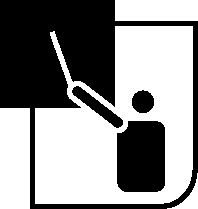
\includegraphics[width=0.75cm]{col11305.imgs/summary_presentation.png} &   \end{array} $ \hspace{2 pt}\raisebox{-5 pt}{} {(section shortcode: P10017 )} \par 
%     \label{m38730*cid5}
%             \subsection{ The Kinetic Theory of Matter}
%             \nopagebreak
      \label{m38730*id308618}The \textbf{kinetic theory of matter} helps us to explain why matter exists in different \textsl{phases} (i.e. solid, liquid and gas), and how matter can change from one phase to the next. The kinetic theory of matter also helps us to understand other properties of matter. It is important to realise that what we will go on to describe is only a \textsl{theory}. It cannot be proved beyond doubt, but the fact that it helps us to explain our observations of changes in phase, and other properties of matter, suggests that it probably is more than just a theory.
\par 
      \label{m38730*id308641}Broadly, the Kinetic Theory of Matter says that:
\par 
      \label{m38730*id308647}\begin{itemize}[noitemsep]
            \label{m38730*uid34}\item Matter is made up of \textbf{particles} that are constantly moving.
\label{m38730*uid35}\item All particles have \textbf{energy}. Solid particles have the least amount of energy and gas particles have the greatest amount of energy.
\label{m38730*uid36}\item The \textbf{temperature} of a substance is a measure of the \textsl{average kinetic energy} of the particles.
\label{m38730*uid37}\item A change in \textbf{phase} may occur when the energy of the particles is changed.
\label{m38730*uid38}\item There are \textbf{spaces} between the particles of matter.
\label{m38730*uid39}\item There are \textbf{attractive forces} between particles and these become stronger as the particles move closer together.
\end{itemize}
      \label{m38730*id308767}Table \ref{tab:microscopic:kinetic theory} summarises the characteristics of the particles that are in each phase of matter.\par 
    % \textbf{m38730*uid40}\par
\begin{table}[h]
\begin{center}
\caption{Table summarising the general features of solids, liquids and gases.}
\label{tab:microscopic:kinetic theory}
\begin{tabular}{|p{3cm}|p{3cm}|p{3cm}|p{3cm}|}\hline
\textbf{Property of matter} & \textbf{Solid} & \textbf{Liquid} & \textbf{Gas} \\\hline
Particles & Atoms or molecules & Atoms or molecules & Atoms or molecules \\\hline
Energy and movement of particles & Low energy - particles vibrate around a fixed point & Particles have more energy than in the solid phase & Particles have high energy and are constantly moving  \\\hline
Spaces between particles & Very little space between particles. Particles are tightly packed together & Bigger spaces than in solids & Large spaces because of high energy  \\\hline
Attractive forces between particles & Very strong forces. Solids have a fixed volume. & Weaker forces than in solids, but stronger forces than in gases & Weak forces because of the large distance between particles  \\\hline
Changes in phase & Solids become liquids or gases if their temperature is increased. & A liquid becomes a gas if its temperature is increased. It becomes a solid if its temperature decreases. & In general a gas becomes a liquid or solid when it is cooled. Particles have less energy and therefore move closer together so that the attractive forces become stronger, and the gas becomes a liquid or a solid.  \\\hline
\end{tabular}
\end{center}
\end{table}
    \par
%       \label{m38730*eip-933}The following presentation is a brief summary of the above. Try to fill in the blank spaces before clicking onto the next slide.
    \setcounter{subfigure}{0}
	\begin{figure}[H] % horizontal\label{m38730*slidesharefigure}
    \label{m38730*slidesharemedia}\label{m38730*slideshareflash}\raisebox{-5 pt}{ 
\includegraphics[width=0.5cm]{col11305.imgs/summary_www.png}} { (Presentation:  P10018 )}
      \vspace{2pt}
    \vspace{.1in}
 \end{figure}       \par 
\begin{figure}[H]
\begin{center}
\begin{pspicture}(0,0)(10,2.6)
\SpecialCoor
%\psgrid[gridcolor=lightgray]

\rput(0,0.5){\psframe(0,0)(3,2)
\rput(0.1,0){\multirput(0.2,0.2)(0.4,0){7}{\pscircle(0,0){0.2}}
\multirput(0.4,0.55)(0.4,0){6}{\pscircle(0,0){0.2}}
\multirput(0.2,0.9)(0.4,0){7}{\pscircle(0,0){0.2}}}}

\rput(3.5,0.5){\psframe(0,0)(3,2)
\rput(0.2,0.2){\pscircle(0,0){0.2}}
\rput(0.6,0.3){\pscircle(0,0){0.2}}
\rput(1.2,0.3){\pscircle(0,0){0.2}}
\rput(1.7,0.2){\pscircle(0,0){0.2}}
\rput(2.3,0.3){\pscircle(0,0){0.2}}
\rput(2.8,0.2){\pscircle(0,0){0.2}}
\rput(0.3,0.9){\pscircle(0,0){0.2}}
\rput(0.8,0.7){\pscircle(0,0){0.2}}
\rput(1.5,0.8){\pscircle(0,0){0.2}}
\rput(2.0,0.8){\pscircle(0,0){0.2}}
\rput(2.5,0.7){\pscircle(0,0){0.2}}}

\rput(7,0.5){\psframe(0,0)(3,2)
\rput(2.5,0.5){\pscircle(0,0){0.2}}
\rput(2.4,1.7){\pscircle(0,0){0.2}}
\rput(1.5,1){\pscircle(0,0){0.2}}
\rput(0.7,1.7){\pscircle(0,0){0.2}}
\rput(0.3,0.3){\pscircle(0,0){0.2}}}

\uput[d](1.5,0.5){solid}
\uput[d](5,0.5){liquid}
\uput[d](8.5,0.5){gas}

\end{pspicture}
\end{center}
\caption{The three phases of matter}
\label{fig:threephases}
\end{figure}
      \label{m38730*id309053}Taking copper as an example we find that in the solid phase the copper atoms have little energy. They vibrate in fixed positions. The atoms are held closely together in a regular pattern called a \textsl{lattice}. If the copper is heated, the energy of the atoms increases. This means that some of the copper atoms are able to overcome the forces that are holding them together, and they move away from each other to form \textsl{liquid copper}. This is why liquid copper is able to flow, because the atoms are more free to move than when they were in the solid lattice. If the liquid is heated further, it will become a gas. Gas particles have lots of energy and are far away from each other. That is why it is difficult to keep a gas in a specific area! The attractive forces between the particles are very weak. Gas atoms will fill the container they are in. Figure \ref{fig:PhaseChanges} shows the changes in phase that may occur in matter, and the names that describe these processes.\par 
    \setcounter{subfigure}{0}
    
\begin{activity}{The three phases of water}
\begin{minipage}{0.5\textwidth}
Water can be in the form of steam, water liquid or ice. Use marbles (or playbough or clay rolled in little balls) to represent water molecules. Arrange the marbles to show the three phases of water. Discuss the properties of each of the phases and the processes and energy in changing from the one phase to the other. 
\end{minipage}
\begin{minipage}{.5\textwidth}
\begin{center}
 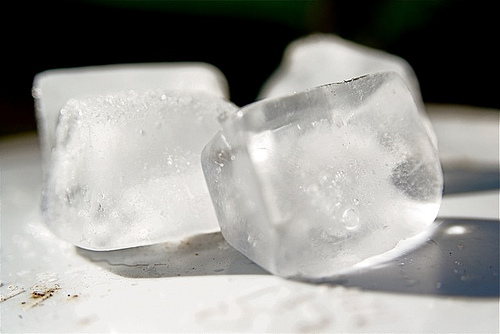
\includegraphics[width=.3\textwidth]{photos/iceby-stevendepolo-flickr.jpg}\par
\textit{Picture by stevendepolo on Flickr.com}
\end{center}
\begin{center}
 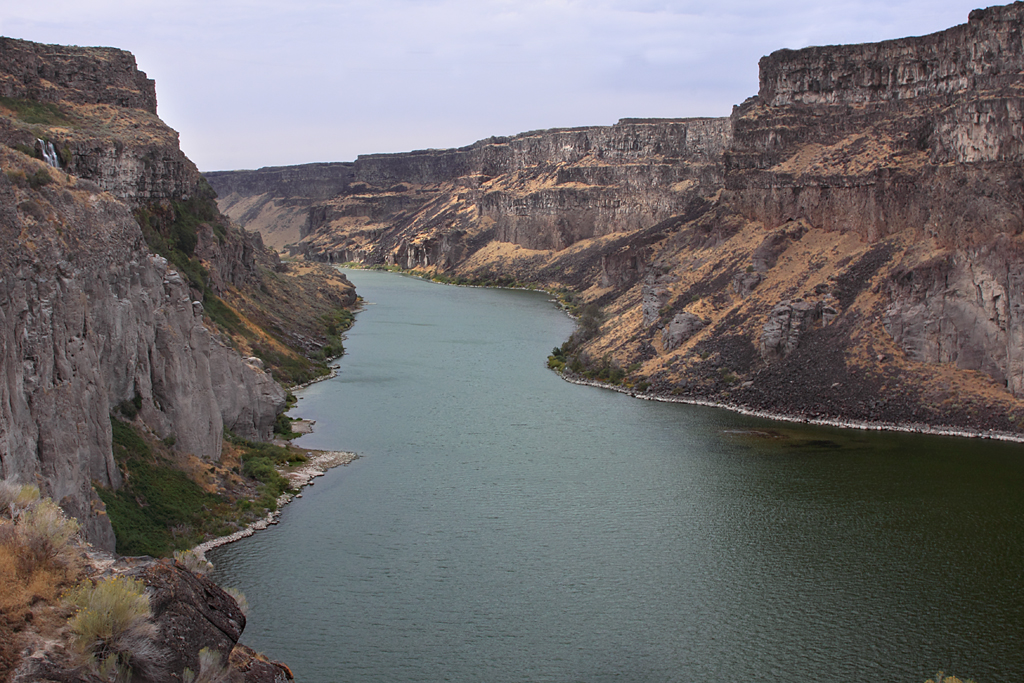
\includegraphics[width=.3\textwidth]{photos/AlanVernon.jpg}\par
\textit{Picture by Alan Vernon on Flickr.com}
\end{center}
\end{minipage}
\end{activity}

      
\label{m38730*cid7}
            \section{Summary}
            \nopagebreak
\label{m38730*id311034}\begin{itemize}[noitemsep]
            \label{m38730*id973}\item There are three states of matter: solid, liquid and gas.\label{m38730*id872}\item Diffusion is the movement of particles from a high concentration to a low concentration. Brownian motion is the diffusion of many particles.\label{m38730*uid80}\item The \textbf{kinetic theory of 
matter} attempts to explain the behaviour of matter in different 
phases.
\label{m38730*uid81}\item The kinetic theory of matter says that all matter is 
composed of \textbf{particles} which have a certain 
amount of \textbf{energy} which allows them to 
\textbf{move} at different speeds depending on the 
temperature (energy). There are \textbf{spaces} 
between the particles and also \textbf{attractive 
forces} between particles when they come close together.
\label{m38730*uid83}\item \textbf{Melting point} is the 
temperature at which a \textsl{solid} changes its 
phase to become a \textsl{liquid}. The reverse 
process (change in phase from liquid to solid) is called \textbf{freezing}.
\label{m38730*uid84}\item \textbf{Boiling point} is the 
temperature at which a liquid changes phase to become a gas. The reverse 
process (change in phase from gas to liquid) is called \textbf{condensing}. 
\end{itemize}
\label{m38730*cid9}
            \begin{eocexercises}{States of matter and the kinetic molecular theory}
            \nopagebreak \noindent
\label{m38730*id311490}\begin{enumerate}[noitemsep, label=\textbf{\arabic*}. ] 
            \label{m38730*uid87}\item Give one word or term for each of the following 
descriptions.
\label{m38730*id311506}\begin{enumerate}[noitemsep, label=\textbf{\alph*}. ] 
            \label{m38730*uid88}\item The change in phase from a solid to a gas.
\label{m38730*uid89}\item The change in phase from liquid to gas.
\end{enumerate}
                \label{m38730*uid103}\item Water has a boiling point of $100 ^{\circ} C$
\label{m38730*id311744}\begin{enumerate}[noitemsep, label=\textbf{\alph*}. ] 
            \label{m38730*uid104}\item Define 'boiling point'.
\label{m38730*uid105}\item What change in phase takes place when a liquid reaches 
its boiling point?
\label{m38730*uid107}\item Use the kinetic theory of matter and your knowledge of 
intermolecular forces to explain why water changes phase at this temperature.
\end{enumerate}
\label{m38730*id762}\item Describe a solid in terms of the kinetic molecular theory. \newline
            \label{m38730*uid108}\item Refer to the table below which gives the melting and 
boiling points of a number of elements and then answer the questions that follow. (\textsl{Data from http://www.chemicalelements.com})
    % \textbf{m38730*id311817}\par
          \begin{table}[H]
    % \begin{table}[H]
    % \\ 'id2883166' '1'
        \begin{center}
      \label{m38730*id311817}
      \begin{tabular}{|l|l|l|}\hline
\textbf{Element} & \textbf{Melting point ($^{\circ} \text{C}$)} & \textbf{Boiling point ($^{\circ} \text{C}$)} \\ \hline
        copper &
        1083 &
        2567 \\ \hline
        magnesium &
        650 &
        1107 \\ \hline
        oxygen &
        -218,4 &
        -183 \\ \hline
        carbon &
        3500 &
        4827 \\ \hline
        helium &
        -272 &
        -268,6 \\ \hline
        sulphur &
        112,8 &
        444,6 \\ \hline
    \end{tabular}
      \end{center}
\end{table}
  \label{m38730*id312057}\begin{enumerate}[noitemsep, label=\textbf{\alph*}. ] 
            \label{m38730*uid109}\item What state of matter (i.e. solid, liquid or gas) will each of 
these elements be in at room temperature ($25^{\circ} \text{C}$)?
\label{m38730*uid110}\item Which of these elements has the strongest forces 
between its atoms? Give a reason for your answer.
\label{m38730*uid111}\item Which of these elements has the weakest forces between 
its atoms? Give a reason for your answer.
\end{enumerate}
\item Complete the following submicroscopic diagrams to show what magnesium will look like in the solid, liquid and gas phase.
\begin{figure}[H]
\begin{center}
\scalebox{.8}{
\begin{pspicture}(0,0)(10,2.6)
\SpecialCoor
%\psgrid[gridcolor=lightgray]

\rput(0,0.5){\psframe(0,0)(3,2)}

\rput(3.5,0.5){\psframe(0,0)(3,2)}

\rput(7,0.5){\psframe(0,0)(3,2)}

\uput[d](1.5,0.5){solid}
\uput[d](5,0.5){liquid}
\uput[d](8.5,0.5){gas}

\end{pspicture}
}
\end{center}
\end{figure}
                \end{enumerate}
\label{m38730**end}
  \label{3fc6acf7f608d0b0e2d136d6a7710402**end}
\par \raisebox{-5 pt}{
\includegraphics[width=0.5cm]{col11305.imgs/summary_www.png}} Find the answers with the shortcodes:
 \par \begin{tabular}[h]{cccccc}
 (1.) l2t  &  (2.) lip  &  (3.) lim  &  (4.) lgf  &  (5.) liy  & \end{tabular}
\end{eocexercises}